\chapter{Diseño e implementación} % Main chapter title

\label{Chapter3} % Change X to a consecutive number; for referencing this chapter elsewhere, use \ref{ChapterX}

Este capítulo aborda el proceso de construcción del sistema de recomendación, desde la concepción de la solución hasta su materialización en un entorno operativo. Se presentan las principales decisiones de diseño, el tratamiento de los datos y las técnicas empleadas para generar las recomendaciones, así como los lineamientos seguidos para asegurar que la propuesta resulte escalable, reproducible y alineada con los objetivos del negocio.

%----------------------------------------------------------------------------------------

\section{Diseño de solución}

El sistema de recomendación se diseñó con el objetivo de estimar la afinidad entre clientes y productos en un entorno caracterizado por alta escala, heterogeneidad de perfiles y rotación constante del portafolio. El diseño de la solución se apoyó en una arquitectura en capas que permite integrar diversas fuentes de datos, transformarlas en estructuras analíticas consistentes, entrenar modelos capaces de capturar relaciones complejas y, finalmente, desplegar las recomendaciones en un flujo operativo estable y reproducible.

La primera capa corresponde a la ingestión de datos, instancia en la que se integran registros transaccionales, interacciones digitales y atributos contextuales. Los datos transaccionales reflejan las compras efectivas realizadas en distintos horizontes temporales, lo que aporta evidencia directa sobre las preferencias observadas. Las interacciones digitales, en cambio, ofrecen señales implícitas de interés a partir de búsquedas, visualizaciones de productos o modificaciones en el carrito. Finalmente, los atributos contextuales caracterizan tanto a los clientes, mediante variables asociadas a su canal de comercialización, localización o tamaño, como a los productos, a partir de propiedades como marca, categoría o segmento.

La segunda capa se orienta a la preparación de los datos. En esta etapa se construyen las matrices de interacciones cliente–producto y se generan representaciones temporales que permiten capturar la dinámica de la demanda. Asimismo, se aplican técnicas de tratamiento de valores faltantes y de codificación de atributos categóricos, con el fin de asegurar consistencia y compatibilidad entre las distintas fuentes. El resultado de este proceso es un conjunto de estructuras homogéneas que sientan las bases para la etapa de modelado.

El modelado constituye la tercera capa de la arquitectura. En este punto se combinan distintos enfoques con el fin de maximizar la capacidad predictiva y superar las limitaciones de cada técnica individual. El filtrado colaborativo implícito, implementado a través de factorización matricial con el método ALS, permite capturar patrones latentes a partir de historiales de compra extensos. Los modelos basados en contenido complementan este enfoque al aprovechar descripciones de clientes y productos, y ofrecen una alternativa frente al problema del arranque en frío. Adicionalmente, se exploran modelos híbridos y de aprendizaje profundo capaces de integrar simultáneamente señales transaccionales y digitales, y de modelar relaciones no lineales entre las variables.

Finalmente, la capa de despliegue asegura la integración del motor de recomendación en el ecosistema tecnológico de la empresa. El pipeline resultante genera listas de productos priorizados para cada cliente, incorpora mecanismos de versionado y monitoreo de modelos, y permite evaluar su desempeño en forma continua. De este modo, la solución se diseñó no solo para alcanzar precisión en la generación de recomendaciones, sino también para garantizar escalabilidad, reproducibilidad y adaptabilidad frente a la evolución del portafolio y a los cambios en los objetivos estratégicos.

La arquitectura de la solución se representa en la figura \ref{fig:arquitectura}. Allí se observa el flujo general del sistema, desde la integración de datos hasta la generación de recomendaciones. El diagrama sintetiza los módulos principales y sus interacciones, y ofrece una visión global que facilita comprender cómo se organiza el motor de afinidad.

\begin{figure}[H]
  \centering
  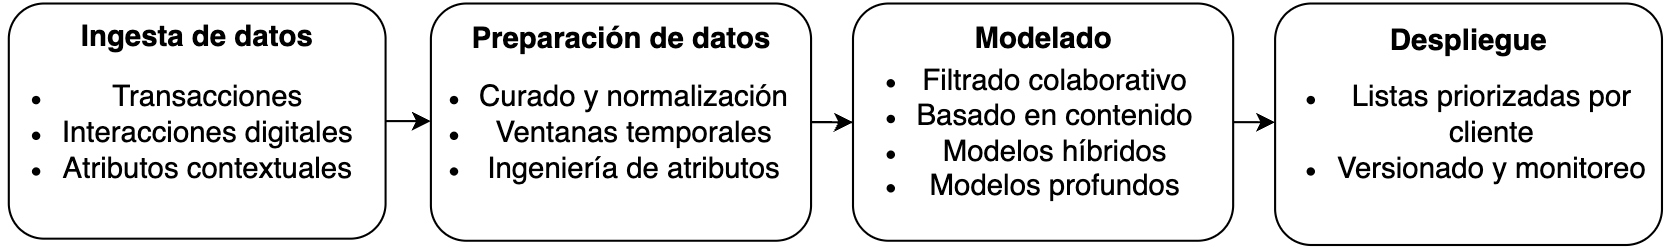
\includegraphics[width=0.9\textwidth]{Figures/Arquitectura.png}
  \caption{Arquitectura de alto nivel del sistema de recomendación.}
  \label{fig:arquitectura}
\end{figure}

%----------------------------------------------------------------------------------------

\section{Preparación de los datos}

La preparación de los datos se centró en transformar las distintas fuentes disponibles en insumos consistentes y comparables para el entrenamiento de los modelos de recomendación. El proceso partió de tres conjuntos principales de información: registros transaccionales, eventos digitales generados en la aplicación y atributos contextuales de clientes y productos. La combinación de estas fuentes permitió construir una representación integral de la relación cliente–producto, en la que se entrelazan tanto preferencias explícitas como señales implícitas de interés.

Los registros transaccionales se encontraban a nivel de operación individual, con granularidad diaria y asociados a identificadores de cliente, producto, cantidad y monto. Este tipo de información es particularmente relevante en entornos de consumo masivo B2B, donde suele observarse una fuerte concentración de las compras en un subconjunto reducido de productos y clientes. De manera preliminar, se advierte un patrón cercano a la regla de Pareto \cite{BOOK:Koch1998}, un pequeño grupo de marcas concentra la mayor parte del volumen mientras que muchos otros artículos registran ventas esporádicas. Esta característica, común en el sector, anticipa la necesidad de abordar los sesgos hacia productos de alta rotación en etapas posteriores del análisis.

Los eventos digitales, por su parte, se encontraban a nivel de interacción, con registros de búsquedas, visualizaciones, adiciones y remociones en el carrito, y clics en promociones. Estos datos permiten capturar señales tempranas de interés que no siempre se traducen en transacciones. No obstante, su naturaleza los hace sensibles al ruido: interacciones aisladas, comportamientos exploratorios o promociones masivas pueden generar señales que no representan un patrón estable. En consecuencia, aunque aportan cobertura y diversidad, requieren una interpretación cuidadosa para evitar que se sobreestimen comportamientos circunstanciales.

Finalmente, los atributos contextuales ofrecieron información complementaria a nivel de cliente y producto. En el caso de los clientes, la granularidad fue de punto de venta, con variables que reflejan diferencias de canal, localización o tamaño, factores que suelen condicionar significativamente las decisiones de compra. En el caso de los productos, los atributos de marca, segmento, envase o rango de precio permiten distinguir entre artículos de consumo masivo y aquellos de carácter más selectivo, lo que introduce heterogeneidad que no siempre se refleja en los registros transaccionales.

La integración de estas fuentes en un repositorio unificado aseguró la compatibilidad de identificadores y la alineación temporal de los registros, lo que habilitó su uso conjunto en el análisis. Las primeras observaciones sugieren un escenario donde coexisten concentración de la demanda en pocos productos y clientes, señales digitales útiles pero ruidosas y una marcada diversidad contextual. Estos fenómenos, característicos del consumo masivo B2B, definen los ejes que serán explorados en mayor detalle durante el análisis exploratorio y que posteriormente condicionarán las decisiones de ingeniería de atributos y modelado.

%----------------------------------------------------------------------------------------

\section{Análisis exploratorio de los datos}

El análisis exploratorio constituye una etapa fundamental para comprender la estructura y los patrones subyacentes en la información disponible antes de su utilización en modelos de recomendación. Su objetivo es identificar distribuciones, tendencias y relaciones entre variables que permitan caracterizar el comportamiento de los clientes y del portafolio de productos, así como anticipar posibles limitaciones o sesgos que afecten el desempeño de los algoritmos.

En esta sección se examinan distintas dimensiones de los datos, e incluye la concentración de clientes y productos, la diversidad de los portafolios de compra, las correlaciones entre variables transaccionales y digitales, y la presencia de sesgos asociados a la popularidad.Este análisis preliminar no solo proporciona una visión descriptiva del conjunto de datos, sino que también orienta decisiones posteriores de ingeniería de atributos y diseño de modelos, al revelar qué señales resultan más informativas y qué fenómenos requieren un tratamiento específico.

\subsection{Curvas de concentración de clientes y productos}

El análisis de concentración constituye un paso clave para comprender la distribución del consumo en entornos de negocio masivo. La figura \ref{fig:concentracion_productos} muestra la curva de concentración de productos, donde se observa que un reducido conjunto concentra la mayor parte del volumen total. En particular, el 20\% de los productos explica cerca del 90\% de las ventas acumuladas, mientras que el resto conforma una extensa cola larga con niveles de rotación significativamente menores. Este comportamiento coincide con la ley de Pareto o principio 80/20 \cite{BOOK:Koch1998}, ampliamente documentado en mercados de consumo masivo, donde la dinámica competitiva se organiza en torno a un pequeño núcleo de artículos de alta popularidad y una mayoría de baja incidencia \cite{BOOK:Anderson2006}.

\begin{figure}[htpb]
	\centering
	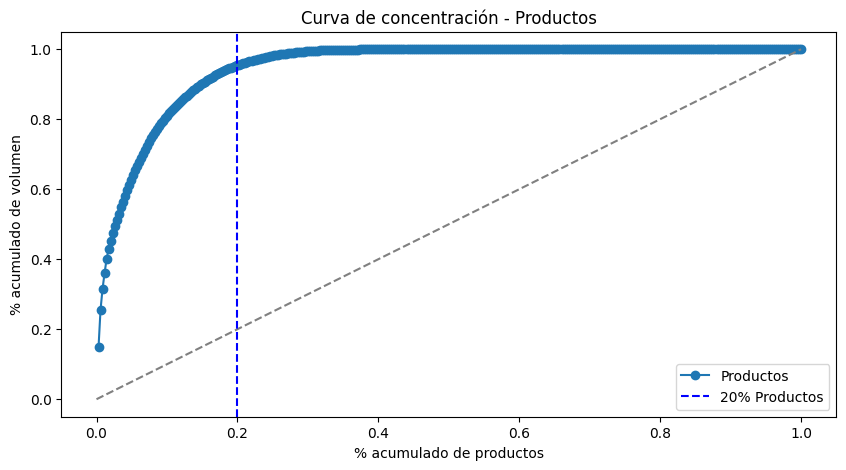
\includegraphics[scale=.55]{./Figures/concentracion_productos.png}
	\caption{Concentración de productos en el portafolio.}
	\label{fig:concentracion_productos}
\end{figure}

De manera análoga, la figura \ref{fig:concentracion_clientes} refleja la concentración del consumo en la base de clientes. Los resultados indican que cerca del 20\% de los puntos de venta generan alrededor del 80\% del volumen total, lo que pone de manifiesto la existencia de clientes estratégicos que concentran gran parte de la demanda. Esta distribución desigual plantea desafíos relevantes para el diseño de sistemas de recomendación, ya que las señales provenientes de clientes de alto volumen tienden a dominar los modelos, lo que genera sesgos hacia productos y comportamientos mayoritarios.

\begin{figure}[htpb]
	\centering
	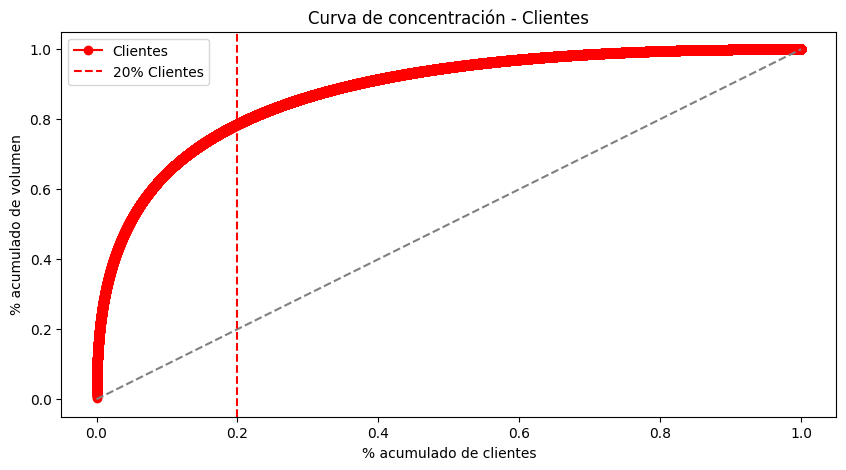
\includegraphics[scale=.55]{./Figures/concentracion_clientes.png}
	\caption{Concentración de clientes.}
	\label{fig:concentracion_clientes}
\end{figure}

La evidencia empírica confirma así que tanto el portafolio de productos como la base de clientes presentan fuertes patrones de concentración. En consecuencia, un motor de recomendación que busque maximizar su impacto no solo debe capturar la afinidad entre clientes y productos más relevantes, sino también considerar mecanismos que favorezcan la diversidad y la exploración de la cola larga. Esta perspectiva resulta fundamental para equilibrar la explotación de los artículos de mayor rotación con la exposición de productos menos populares, lo que alinea los objetivos de negocio con la mejora de la experiencia del cliente.

\subsection{Patrones de diversidad en el portafolio}

El análisis de la diversidad en el portafolio de productos por cliente permite comprender la amplitud y heterogeneidad de los hábitos de consumo. La figura \ref{fig:hist_diversidad} muestra la distribución del número de productos distintos adquiridos por cliente en un mes. Los resultados evidencian que la mayoría de los puntos de venta concentra su demanda en un conjunto reducido de referencias, mientras que un número menor incorpora una mayor amplitud de marcas y presentaciones. Esta asimetría confirma la coexistencia de clientes de bajo rango de exploración con otros de portafolio más diversificado.

\begin{figure}[htpb]
	\centering
	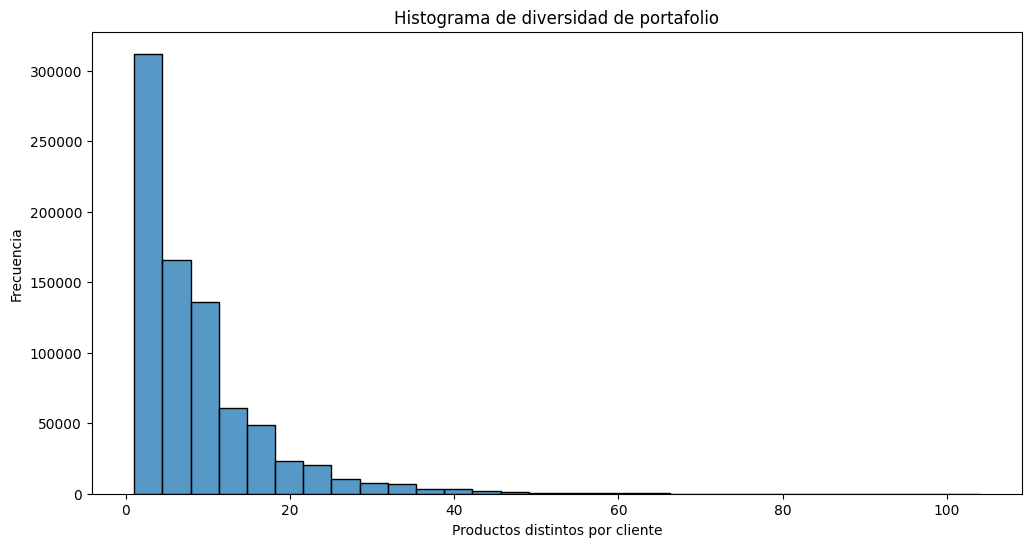
\includegraphics[scale=.52]{./Figures/hist_diversidad.png}
	\caption{Histograma de diversidad de portafolio: número de productos distintos por cliente.}
	\label{fig:hist_diversidad}
\end{figure}

Las diferencias se acentúan al segmentar por canal comercial, como se puede apreciar en la figura \ref{fig:boxplot_diversidad}. En este caso, se observa que los autoservicios tienden a manejar un surtido más amplio de productos en comparación con kioscos y tiendas tradicionales, lo que refleja el rol que cada formato cumple dentro de la red de distribución. Este hallazgo es consistente con la literatura en consumo masivo, que indica que la variedad de portafolio suele estar asociada a factores estructurales como el tamaño del punto de venta y la frecuencia de reposición \cite{BOOK:Kotler2017}.

\begin{figure}[htpb]
	\centering
	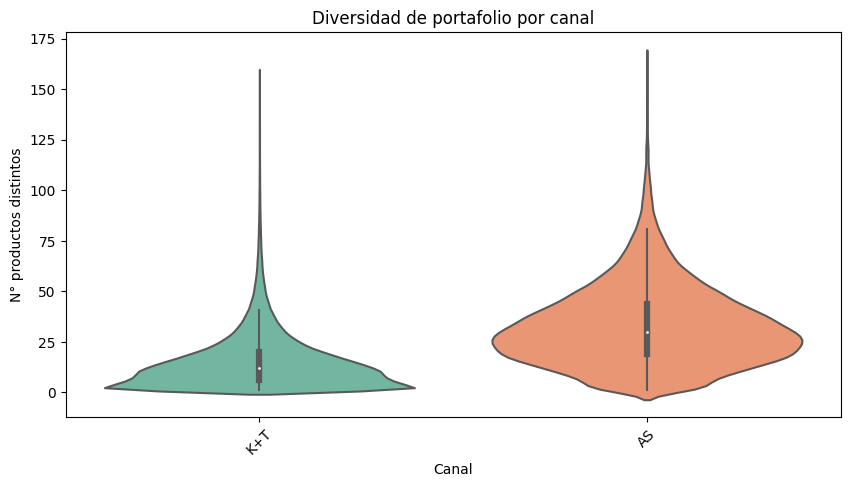
\includegraphics[scale=.6]{./Figures/boxplot_diversidad_canal.png}
	\caption{Diversidad de portafolio segmentada por canal comercial.}
	\label{fig:boxplot_diversidad}
\end{figure}

La figura \ref{fig:log_log_plot} ilustra el fenómeno de concentración extrema en la demanda, donde unos pocos productos acumulan la mayoría de los pedidos mientras que la gran mayoría registra volúmenes marginales. Para representar este patrón se utiliza un \textit{log–log plot}, en el cual tanto el ranking de los productos como su número total de pedidos se expresan en escala logarítmica. Esta transformación permite visualizar con mayor claridad distribuciones de tipo cola larga, que en escalas lineales suelen quedar ocultas por la presencia de artículos extremadamente populares. El gráfico muestra una pendiente decreciente que confirma la existencia de este comportamiento: un reducido conjunto de productos concentra un volumen muy elevado, mientras que el resto se distribuye en la larga cola de baja rotación.

Este patrón no solo refuerza la evidencia presentada en las curvas de concentración, sino que además resalta un sesgo estructural que enfrenta cualquier sistema de recomendación en entornos de consumo masivo. Al entrenarse sobre datos históricos, los modelos tienden de manera natural a privilegiar los productos más populares, lo que reproduce el sesgo de popularidad y reduce la diversidad de las sugerencias. Este fenómeno señala la tensión entre explotación de productos estrella y exploración de la cola larga \cite{BOOK:Celma2010}. En este contexto, el desafío consiste en diseñar mecanismos que permitan balancear ambos extremos, de modo que se garantice relevancia sin sacrificar diversidad ni cobertura.

\begin{figure}[htpb]
	\centering
	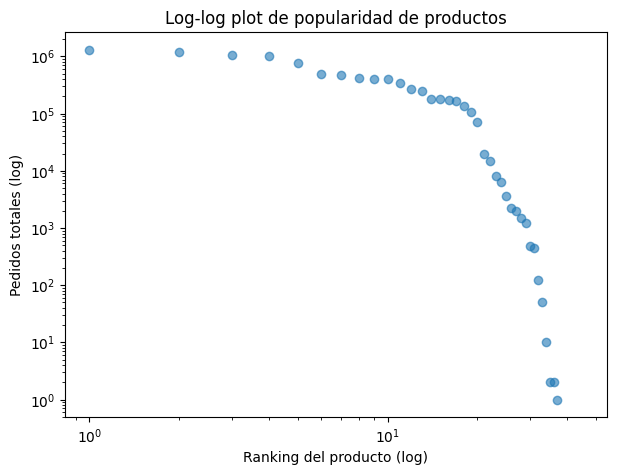
\includegraphics[scale=.65]{./Figures/log_log_plot.png}
	\caption{\textit{Log log plot} de la popularidad de productos.}
	\label{fig:log_log_plot}
\end{figure}

El análisis de co-ocurrencia entre los productos más relevantes, presentado en la figura \ref{fig:heatmap_coocurrencia}, revela patrones de complementariedad en la demanda. Determinadas marcas y presentaciones tienden a aparecer de manera conjunta en los carritos de compra, lo que sugiere asociaciones naturales que pueden ser aprovechadas por un motor de recomendación. Estos resultados refuerzan la importancia de capturar no solo la popularidad individual de cada producto, sino también las relaciones de afinidad que emergen a nivel de portafolio.

\begin{figure}[htpb]
	\centering
	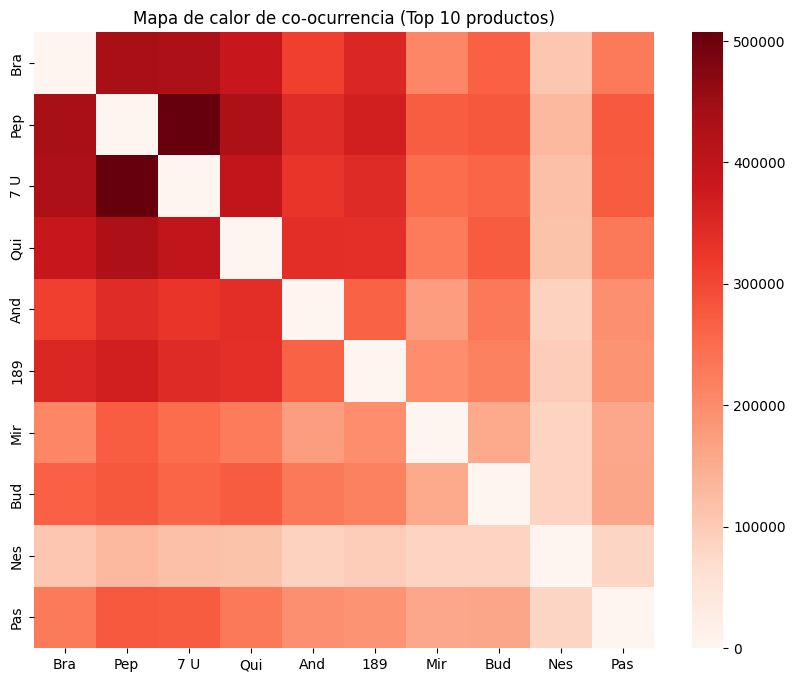
\includegraphics[scale=.5]{./Figures/heatmap_coocurrencia.png}
	\caption{Mapa de calor de co-ocurrencia entre los 10 productos más relevantes.}
	\label{fig:heatmap_coocurrencia}
\end{figure}

\subsection{Correlaciones entre variables transaccionales y digitales}

El análisis de correlaciones busca identificar hasta qué punto las señales digitales anticipan comportamientos de compra y, en consecuencia, evaluar su potencial como insumos predictivos. Con el fin de evaluar la relación entre interacciones digitales y transacciones, se construyó una matriz de correlación entre las principales variables del conjunto de datos, observada en la figura \ref{fig:heatmap_corr}. 

\begin{figure}[htpb]
	\centering
	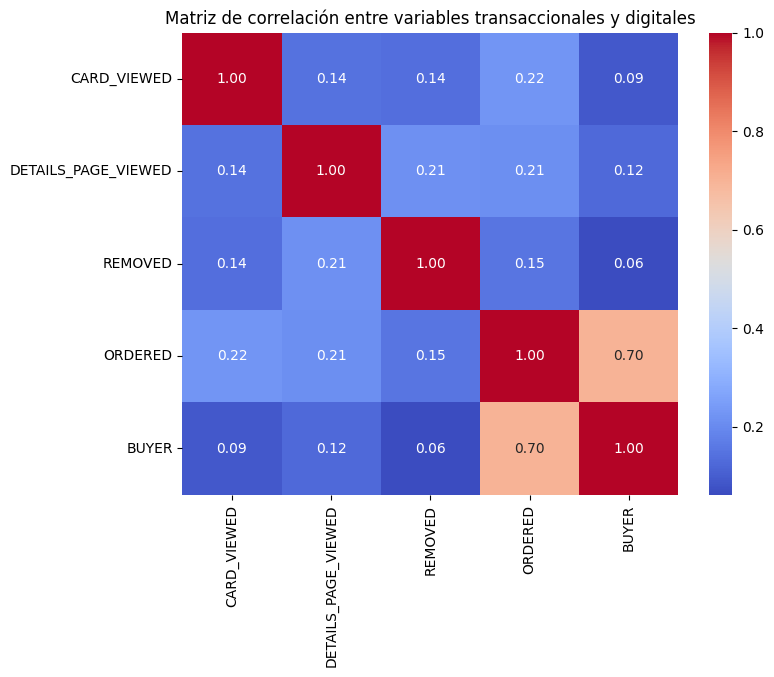
\includegraphics[scale=.55]{./Figures/heatmap_corr.png}
	\caption{Matriz de correlación entre variables transaccionales y digitales.}
	\label{fig:heatmap_corr}
\end{figure}

Los resultados muestran una correlación elevada entre \texttt{ORDERED} y \texttt{BUYER} ($r=0.70$), coherente con el hecho de que ambas variables reflejan distintos aspectos de la misma dimensión de compra. En contraste, las correlaciones de las señales digitales con las variables de compra resultan positivas pero de menor magnitud: \texttt{CARD\_VIEWED} y \texttt{DETAILS\_PAGE\_VIEWED} muestran coeficientes bajos, lo que indica que la exposición y exploración de productos acompaña el proceso de compra, aunque no lo determina. La variable \texttt{REMOVED} presenta la relación más débil, lo que sugiere que los eventos de descarte contienen información ruidosa y limitada respecto de la propensión a comprar.

La correlación contemporánea entre interacciones digitales y compras confirma que las transacciones pasadas siguen siendo el principal indicador de comportamiento, mientras que las señales digitales aportan evidencia complementaria que, si bien débil de manera aislada, resulta relevante al integrarse en un modelo híbrido.

Con el fin de explorar la capacidad predictiva de estas variables, se calculó la correlación de cada una con la compra del mismo cliente–producto en el mes siguiente. Los resultados, en la figura \ref{fig:corr_prox_mes},  muestran que las transacciones pasadas (\texttt{BUYER}, \texttt{ORDERED}) son los predictores más fuertes, aunque las señales digitales también aportan información incremental. En particular, la variable \texttt{CARD\_VIEWED} presenta un coeficiente relevante, lo que respalda la hipótesis de que la exposición reiterada a un producto incrementa la probabilidad de recompra.

\begin{figure}[htpb]
	\centering
	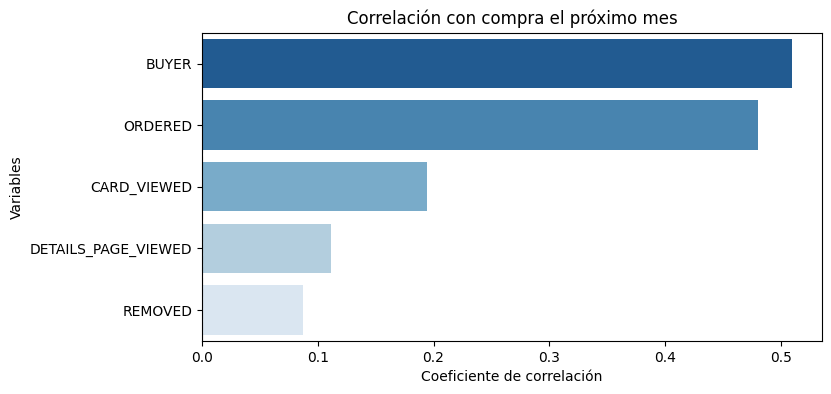
\includegraphics[scale=.6]{./Figures/corr_prox_mes.png}
	\caption{Correlación de variables con la compra en el mes siguiente.}
	\label{fig:corr_prox_mes}
\end{figure}

Finalmente, se evaluó la tasa de recompra según la combinación de señales observadas en meses previos, en la tabla \ref{tab:tasa_recompra}. Los clientes que registran tanto interacción como transacción presentan la mayor tasa de recompra (58,8\%), seguidos por aquellos con solo órdenes (44,1\%). En contraste, quienes solo exhiben interacciones digitales alcanzan un nivel considerablemente menor (17,6\%), incluso por debajo del grupo sin ningún registro previo (28,3\%). Este resultado sugiere que las interacciones aisladas no constituyen un predictor confiable de recompra, sino que tienden a reflejar un interés superficial que rara vez se traduce en pedidos. En cambio, la combinación de transacciones previas con señales digitales se confirma como el escenario de mayor poder explicativo, ya que aprovecha la solidez de la evidencia transaccional y, al mismo tiempo, permite mejorar la capacidad de anticipar comportamientos futuros en casos donde no existen registros abundantes de compra.

\begin{table}[h]
	\centering
	\caption[Tasa de recompra por combinación de señales]{Tasa de recompra según la combinación de señales previas.}
	\label{tab:tasa_recompra}
	\begin{tabular}{l c}    
		\toprule
		\textbf{Grupo}     & \textbf{Tasa de recompra}\\
		\midrule
		Interacción y orden & 58{,}79 \% \\
		Solo orden & 44{,}05 \% \\
		Ninguno & 28{,}30 \% \\
		Solo interacción & 17{,}64 \% \\
		\bottomrule
	\end{tabular}
\end{table}

\subsection{Observaciones preliminares del análisis exploratorio}

El análisis exploratorio permitió identificar una serie de patrones que resultan fundamentales para orientar el diseño del motor de recomendación. En primer lugar, se confirmó que tanto el portafolio de productos como la base de clientes presentan fuertes niveles de concentración: un reducido conjunto explica la mayor parte del volumen, mientras que la mayoría se distribuye en una extensa cola larga de baja rotación. Este comportamiento introduce un sesgo hacia popularidad que los modelos deben manejar para no sacrificar diversidad \cite{BOOK:Anderson2006}.

En segundo lugar, se observó que la diversidad en los portafolios de compra varía según el tipo de cliente, con autoservicios que incorporan un surtido más amplio en comparación con kioscos y tiendas tradicionales. Además, los análisis de co-ocurrencia revelaron asociaciones frecuentes entre ciertos productos, lo que sugiere la existencia de complementariedades que pueden ser aprovechadas en la generación de recomendaciones.  

En tercer lugar, el estudio de correlaciones entre variables digitales y transaccionales mostró que, si bien las transacciones pasadas constituyen el predictor más sólido de comportamiento, las señales digitales aportan información incremental y se vuelven especialmente relevantes en escenarios de arranque en frío. La evaluación de tasas de recompra confirmó que la combinación de interacciones y compras pasadas es la fuente más robusta de predicción, mientras que las interacciones aisladas presentan un valor explicativo limitado.  

En conjunto, estos hallazgos proporcionan una primera validación de la hipótesis central: la integración de señales transaccionales y digitales, complementadas con atributos contextuales, resulta clave para capturar la heterogeneidad del consumo y diseñar un motor de recomendación capaz de balancear precisión, diversidad y cobertura.

%----------------------------------------------------------------------------------------

\section{Ingeniería de atributos}

La etapa de ingeniería de atributos constituyó uno de los pilares centrales del desarrollo del motor de afinidad, ya que definió la forma en que las distintas fuentes de datos fueron transformadas en representaciones numéricas útiles para los modelos de recomendación. En esta fase se abordó tanto la construcción de la matriz cliente–producto, que sintetiza las interacciones históricas y digitales entre ambas entidades, como la generación de atributos contextuales que describen las características estructurales de clientes y productos.

El objetivo fue capturar la complejidad del comportamiento comercial B2B en consumo masivo, donde coexisten puntos de venta con patrones de compra heterogéneos, portafolios con alta rotación y señales digitales de distinta frecuencia e intensidad. Las fuentes de información se integraron en una arquitectura analítica diseñada para producir variables consistentes, interpretables y estables en el tiempo.

\subsection{Diseño de la matriz cliente–producto}

La matriz cliente–producto constituye el núcleo del sistema de recomendación, ya que representa de forma estructurada las interacciones históricas entre los puntos de venta y el portafolio de productos. Su construcción requirió integrar información transaccional y de comportamiento digital proveniente de la aplicación BEES, transformando ambas fuentes en un conjunto de señales cuantificables que reflejan el nivel de interés o afinidad de cada cliente hacia cada producto.

\subsubsection{Integración de fuentes y depuración de eventos}

Previo a la selección de los eventos a considerar, se realizó un proceso de depuración destinado a eliminar registros residuales o no representativos. Se excluyeron interacciones que no estuvieran asociadas a un producto específico, así como aquellas que correspondían a acciones rutinarias de navegación en la aplicación y que no implicaban una manifestación de preferencia. Este filtrado fue fundamental para reducir el ruido inherente a las señales digitales, un desafío recurrente en sistemas de recomendación donde la actividad exploratoria o automatizada puede superar a la de compra efectiva \cite{BOOK:Ricci2015, ARTICLE:Zhang2019}.

Una vez consolidado el conjunto de eventos válidos, la información se agrupó a nivel mensual por cliente y producto, contabilizando la cantidad de interacciones registradas para cada tipo de evento. Se seleccionaron cuatro categorías principales por su relevancia y consistencia estadística: confirmación de orden (\texttt{ORDERED}), visualización de tarjeta promocional (\texttt{CARD\_VIEWED}), acceso al detalle del producto (\texttt{DETAILS\_PAGE\_VIEWED}) y eliminación del producto del carrito (\texttt{REMOVED}).

Los eventos \texttt{ORDERED} y \texttt{CARD\_VIEWED} cuentan además con subtipos que indican el origen de la recomendación. Por ejemplo, búsquedas populares, club de descuentos, \textit{forgotten items}, pedido fácil, compra incremental o búsquedas recientes. Estos subtipos fueron conservados, dado que reflejan distintos mecanismos de exposición y conversión dentro de la aplicación, y demostraron poseer correlaciones diferenciales con el comportamiento de recompra y con las métricas de desempeño predictivo del modelo.

\subsubsection{Diseño temporal y esquema de ventanas}

El diseño temporal de la matriz responde a la lógica operativa del sistema: las predicciones del mes $N$ deben generarse durante el mes $N-1$, utilizando únicamente información previa. Por ello, se implementó un esquema de ventanas móviles de seis meses, abarcando el período comprendido entre los meses $N-7$ y $N-2$. Dentro de esa ventana se calcularon tres horizontes de observación —último mes, últimos tres meses y últimos seis meses— con el fin de capturar simultáneamente señales recientes y patrones más estables.

A diferencia de los modelos supervisados tradicionales, en los sistemas de recomendación basados en \textit{feedback} implícito no resulta necesario realizar una partición explícita entre conjuntos de entrenamiento y prueba dentro de cada ventana temporal. El objetivo no es predecir una etiqueta conocida, sino aprender representaciones latentes que describan la relación entre clientes y productos. En este contexto, el modelo se entrena utilizando la totalidad de la información disponible hasta el mes previo y se evalúa prospectivamente sobre el siguiente período, replicando las condiciones reales de operación del sistema. Este enfoque, ampliamente recomendado en contextos temporales \cite{ARTICLE:Koren2010,BOOK:Aggarwal2016}, evita el uso de divisiones artificiales que fragmenten el histórico, preserva la coherencia causal y permite aprovechar al máximo los datos recientes para lograr una evaluación más realista del comportamiento futuro.

\subsubsection{Tratamiento y normalizaci\'on de variables}

El conjunto de variables resultante presentaba una alta heterogeneidad en magnitudes, derivada de la coexistencia de clientes con volúmenes de compra muy dispares y productos con distintos niveles de rotación. Esta disparidad podía introducir distorsiones en los cálculos posteriores, en especial en la estimación de distancias y en los procesos de normalización, ya que unos pocos valores extremos tendían a dominar la escala de las variables. Para mitigar este efecto, se aplicó una técnica de \textit{clipping} (\textit{winsorizing}) \cite{BOOK:Aggarwal2015}, que limita los valores por debajo del percentil 1 y por encima del percentil 99, reduciendo la influencia de observaciones atípicas sin alterar la estructura general de los datos. 

Luego, cada variable fue normalizada dentro del grupo cliente–categoría, de modo que representara el peso relativo de un producto sobre el total de la categoría en el portafolio de ese cliente.  Esta forma de estandarización permite que las variables reflejen proporciones comparables entre clientes de distinto tamaño o comportamiento de compra, evitando que las diferencias absolutas de escala o estacionalidad sesguen las medidas de afinidad. En consecuencia, cada \textit{feature} captura la importancia real del producto en relación con el contexto de consumo del cliente, en lugar de su volumen bruto, lo que mejora la capacidad del modelo para generalizar patrones de preferencia.

\subsubsection{Estimación de pesos y generación del score de preferencia}

A partir de estas variables, se definieron pesos específicos para cada tipo de evento y cada ventana temporal, con el fin de obtener un score de preferencia compuesto. La estimación de estos pesos se realizó mediante un proceso de optimización bayesiana con \texttt{Optuna} \cite{ARTICLE:Akiba2019}, maximizando la métrica \textit{Precision@10} sobre un conjunto de validación temporal. Se ejecutaron 100 iteraciones exploratorias, observándose como patrón consistente una mayor ponderación de las señales recientes (1M > 3M > 6M) y una mayor relevancia de los eventos transaccionales respecto de los digitales. Los valores finales de ponderación y los resultados detallados del proceso de optimización se presentan en el apendice \ref{AnexoOptuna}.

\subsubsection{Análisis de la matriz resultante}

El resultado final fue una matriz cliente–producto donde cada celda representa un puntaje implícito de afinidad, obtenido como la combinación ponderada de todas las interacciones entre el cliente y el producto en los distintos horizontes. Esta estructura, de naturaleza dispersa, constituye la base para los algoritmos colaborativos y sirve como punto de partida para el entrenamiento de modelos como \texttt{ALS} y \texttt{LightFM}. 

La matriz resultante comprendió 60{,}2 millones de pares cliente–producto, de los cuales el 13{,}5 \% presentó al menos una interacción registrada, reflejando la típica estructura dispersa de los sistemas de recomendación en entornos de consumo masivo. El score de preferencia exhibió una distribución fuertemente sesgada hacia cero, con un promedio de 0{,}0046 y una desviación estándar de 0{,}0277, lo que indica que la mayoría de las combinaciones poseen niveles de afinidad bajos o nulos. Los percentiles superiores (P90 = 0{,}001; P99 = 0{,}126) confirman que las señales de alta afinidad son poco frecuentes y concentradas en un subconjunto reducido de pares.

Se observó una incidencia de arranque en frío muy acotada: 2{,}981 clientes (1{,}5~\% del total) y un único producto (0{,}54~\% de los ítems) no registraban interacciones en el período de entrenamiento. Este resultado indica una base de datos altamente densa en términos de representatividad de comportamiento, donde casi la totalidad de los clientes y productos posee algún tipo de historial previo. Aun así, la presencia de estos casos justifica la incorporación de componentes basados en contenido dentro del sistema, ya que incluso proporciones pequeñas de usuarios o ítems sin historial pueden impactar en la cobertura global de las recomendaciones \cite{BOOK:Aggarwal2016}.

Al segmentar por comportamiento de compra, los pares con transacción efectiva el proximo mes registraron un score promedio de 0{,}066, muy superior al de aquellos sin compra (0{,}0026), con una correlación de Pearson de 0{,}39 entre ambas variables. Este nivel de asociación, junto con un área bajo la curva ROC (AUC = 0{,}8766), evidencia una sólida capacidad discriminante del score para diferenciar entre pares con y sin compra \cite{BOOK:Ricci2015, ARTICLE:Zhao2022}.

Un resumen de las métricas descriptivas de la matriz se presenta en la tabla~\ref{tab:metricas_matriz}, donde se evidencia su alta dispersión, baja incidencia de casos en arranque en frío y la fuerte correlación entre el score de preferencia y el comportamiento de compra observado. Estas métricas validan que la matriz sintetiza de forma adecuada la estructura latente de preferencias: preserva la dispersión y heterogeneidad propias del dominio, al tiempo que captura la intensidad relativa de las interacciones cliente–producto y su poder explicativo sobre el comportamiento de compra.

\begin{table}[h]
	\centering
	\caption[Métricas descriptivas de la matriz cliente–producto]{Resumen de métricas descriptivas de la matriz cliente–producto.}
	\begin{tabular}{l c}    
		\toprule
		\textbf{Indicador}     & \textbf{Valor}\\
		\midrule
		Total de pares cliente–producto & 60{,}220{,}260 \\
		Densidad de la matriz (\% de celdas no nulas) & 13{,}50 \% \\
		Clientes en arranque en frío & 2{,}981 (1{,}50 \%) \\
		Productos en arranque en frío & 1 (0{,}54 \%) \\
		Media del score de preferencia & 0{,}0046 \\
		Desvío estándar del score & 0{,}0277 \\
		Correlación Buyer–Preference & 0{,}3935 \\
		Área bajo la curva (AUC) & 0{,}8766 \\
		\bottomrule
	\end{tabular}
	\label{tab:metricas_matriz}
\end{table}

\subsection{Diseño de atributos de cliente y producto}

Además de la matriz de interacciones, el sistema de recomendación incorpora un conjunto de atributos específicos de clientes y productos que permiten modelar afinidades a partir de sus características intrínsecas. Estos atributos complementan las señales implícitas y constituyen la base de los enfoques basados en contenido, aportando contexto y capacidad de generalización en escenarios con poca información transaccional o de arranque en frío \cite{BOOK:Ricci2015,BOOK:Aggarwal2016}.

\subsubsection{Construcción de atributos de cliente}

Para los puntos de venta se construyó una representación multicomponente que sintetiza distintos aspectos del comportamiento de compra y del perfil operativo. Las variables derivadas se agruparon en torno a seis dimensiones principales: frecuencia de compra, estabilidad temporal, volumen y crecimiento, diversidad de mix, comportamiento de compra y atributos contextuales. En conjunto, estas dimensiones permiten caracterizar tanto la intensidad como la regularidad y la amplitud del consumo de cada cliente.

La frecuencia de compra se estimó a partir del número de pedidos mensuales, su media y desviación en seis meses, junto con un coeficiente de variación que distingue clientes regulares de aquellos más esporádicos. La estabilidad temporal se midió mediante la variabilidad de las ventas y el volumen transaccionado, incorporando además un indicador binario que identifica clientes estables según su dispersión relativa. El bloque de volumen incluyó métricas acumuladas de ventas y unidades totales, así como el crecimiento del último mes respecto del promedio histórico, utilizado como señal de tendencia reciente. La diversidad del mix se midió a través de la cantidad de marcas, categorías y formatos adquiridos, complementada con un índice de Shannon \cite{ARTICLE:Shannon1948} que resume la concentración de las compras. Por su parte, las variables de comportamiento capturaron la especialización del cliente, por ejemplo, si opera únicamente con cervezas o con bebidas no alcohólicas, la proporción de productos premium en su portafolio, la continuidad de compras en meses consecutivos y la concentración del gasto en las tres principales marcas. Finalmente, las variables contextuales refieren a la geografia y canal, permitiendo diferenciar el comportamiento entre regiones y tipos de punto de venta.

Todas las variables numéricas fueron sometidas a un proceso de \textit{clipping} (\textit{winsorizing}) \cite{BOOK:Aggarwal2015} para reducir la influencia de valores atípicos, seguido de una normalización por \textit{z-score} dentro de los grupos definidos por subregión y canal. Este tratamiento permitió mantener la comparabilidad entre clientes de distinta escala y contexto operativo, evitando que los valores extremos afectaran la calibración de los modelos. Posteriormente, las variables continuas fueron discretizadas en tres niveles mediante cuantiles: bajo, medio y alto. Esto facilita su integración en modelos que utilizan representaciones categóricas o embeddings. Las variables categóricas se estandarizaron y completaron con etiquetas neutras, garantizando la consistencia del conjunto final. El resultado fue un vector descriptivo equilibrado y robusto que combina información transaccional, contextual y comportamental de cada cliente.

\subsubsection{Construcción de atributos de producto}

El diseño de atributos de producto siguió una lógica análoga. En este caso, las variables reflejan la posición del producto dentro del portafolio, su desempeño comercial y su nivel de adopción en el mercado. Se incorporaron indicadores de volumen y ventas acumuladas, número de pedidos y clientes alcanzados, crecimiento mensual y ticket promedio. La penetración se estimó como la proporción de clientes que adquirieron el producto en el período, mientras que la recurrencia representó la frecuencia media de recompra entre los compradores. También se midieron la diversificación geográfica y de canal y la composición por unidad de negocio (\texttt{CZA} o \texttt{NABS}), junto con atributos estructurales como segmento de marca, tipo de envase y condición de producto premium. Finalmente, se calcularon métricas relativas de desempeño, como la participación del producto dentro de su categoría o su marca, y un índice de diversidad de clientes que resume la dispersión del gasto a través de distintos puntos de venta.

El procesamiento estadístico aplicado a los productos replicó la metodología utilizada para los clientes, combinando \textit{winsorizing} para el tratamiento de valores extremos, normalización por \textit{z-score} dentro de cada unidad de negocio y discretización por cuantiles. De esta forma, se obtuvo una representación homogénea que preserva la comparabilidad entre productos de distinta rotación o escala de ventas.

\subsubsection{Representatividad de los atributos}

Con el propósito de evaluar la representatividad y calidad de la información contenida en los atributos de cliente y producto, se desarrolló un análisis exploratorio basado en métricas estadísticas y geométricas, en lugar de un modelo predictivo supervisado. Este procedimiento permitió caracterizar la varianza, la correlación con la ocurrencia de compra y la similitud estructural entre entidades, cuantificando así la diversidad informativa y la capacidad discriminante de cada conjunto de variables.

En el caso de los clientes, se analizaron 95 atributos válidos (59 numéricos y 36 categóricos), tras la conversión automática de variables textuales y la indexación de categorías. Las variables con mayor varianza correspondieron a medidas de volumen y frecuencia, como la facturación total, el número de pedidos y el volumen promedio, lo que refleja la amplia heterogeneidad de los puntos de venta. Las correlaciones más elevadas con la variable de compra se observaron en indicadores de continuidad y madurez, tales como la cantidad de meses consecutivos con actividad y la frecuencia de pedidos, con coeficientes próximos a 0{,}32. La similitud coseno promedio entre representaciones de clientes fue de 0{,}9985, indicando una alta consistencia interna en el espacio de atributos y una concentración de la variabilidad en unas pocas dimensiones relevantes.

En los productos se evaluaron 61 atributos (37 numéricos y 24 categóricos), entre los cuales predominaron las métricas de desempeño y alcance comercial. Las variables con mayor varianza fueron las asociadas al volumen total, la facturación y el número de puntos de venta atendidos, mientras que las correlaciones más fuertes con la variable objetivo correspondieron a la penetración de clientes y a la cobertura comercial, con coeficientes superiores a 0{,}84. La similitud coseno promedio fue de 0{,}6449, evidenciando una mayor dispersión relativa respecto de los clientes, coherente con la diversidad estructural del portafolio.

Para complementar el análisis, se exploró la capacidad de las features de cliente y producto para reflejar diferencias inherentes en los datos mediante una reducción de dimensionalidad con Análisis de Componentes Principales (PCA). El objetivo fue observar si las categorías de negocio se separan naturalmente en el espacio de representación. 

En el caso de los clientes, figura \ref{fig:pca_clientes}, la proyección PCA de los puntos de venta muestra una separación visible entre los canales Autoservicio (AS) y Kiosco + Tradicional (K+T). Si bien existe cierto solapamiento, los autoservicios tienden a concentrarse en la parte superior del plano, mientras que los puntos de venta tradicionales se agrupan hacia zonas inferiores. Esto sugiere que las features de cliente capturan patrones de comportamiento diferenciados entre canales.

\begin{figure}[h]
	\centering
	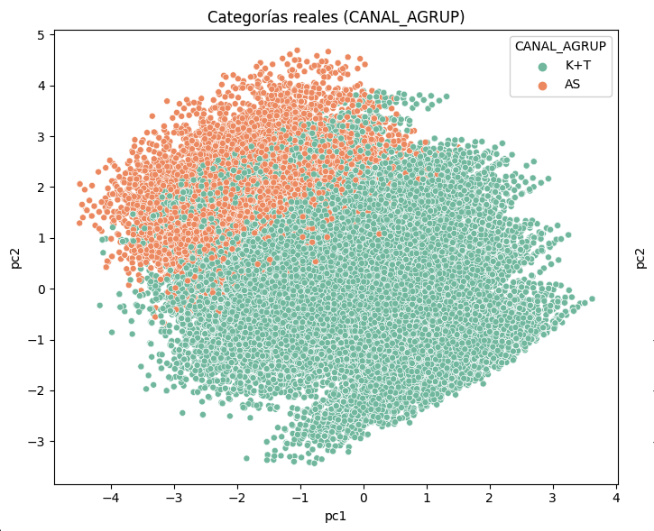
\includegraphics[width=0.9\textwidth]{pca_clientes.png}
	\caption[Proyección PCA de clientes por canal comercial]{Proyección PCA de clientes por canal comercial.}
	\label{fig:pca_clientes}
\end{figure}

En los productos, figura \ref{fig:pca_productos}, la representación revela grupos bien definidos que corresponden a las divisiones Cerveza (CZA), No Alcohólicas (NABS) y Vinos o Adyacencias (Match). Las categorías se ubican en regiones claramente separadas del plano, lo que indica que las variables de producto describen de manera efectiva diferencias estructurales entre líneas de negocio.

\begin{figure}[h]
	\centering
	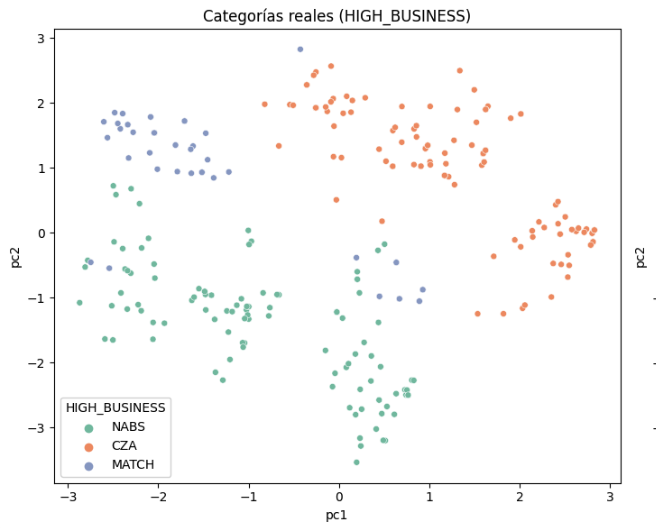
\includegraphics[width=0.9\textwidth]{pca_productos.png}
	\caption[Proyección PCA de productos por línea de negocio]{Proyección PCA de productos por línea de negocio.}
	\label{fig:pca_productos}
\end{figure}

En conjunto, los resultados del PCA demuestran que las features de producto reflejan con claridad la organización natural del portafolio, mientras que las de cliente presentan una diferenciación más moderada pero coherente con los tipos de canal. Ambas representaciones resultan adecuadas para describir la heterogeneidad comercial de la base analizada y aportan una base sólida para su integración en modelos híbridos de recomendación.

%----------------------------------------------------------------------------------------

\section{Desarrollo de modelos}

El desarrollo de los modelos constituye la fase central del sistema de recomendación, donde la matriz cliente–producto construida en etapas previas se transforma en un mecanismo capaz de estimar la afinidad entre ambos. El objetivo es asignar a cada combinación posible un puntaje continuo que refleje la probabilidad relativa de interés, permitiendo ordenar los productos según su relevancia esperada para cada cliente.

Para abordar este desafío se exploraron distintos enfoques de modelado, que combinan estrategias colaborativas, basadas en contenido y de aprendizaje profundo. En primer lugar, se implementó un modelo de filtrado colaborativo mediante el algoritmo \textit{Alternating Least Squares} (ALS) \cite{ARTICLE:ALS2008, ARTICLE:Hu2008}, que aprende representaciones latentes de clientes y productos a partir de los patrones de interacción observados. En segundo lugar, se desarrolló un modelo híbrido con \texttt{LightFM} \cite{ARTICLE:LightFM2015}, capaz de integrar señales colaborativas con atributos explícitos de clientes y productos, mitigando así el problema del arranque en frío.

Complementariamente, se incorporaron dos variantes basadas en redes neuronales. La primera aprende representaciones de clientes y productos a partir de sus atributos mediante arquitecturas de \textit{embeddings} \cite{ARTICLE:Grbovic2018}, que pueden combinarse con ALS en un esquema de ensamble. La segunda corresponde al enfoque de \textit{Neural Collaborative Filtering} (NCF) \cite{ARTICLE:He2017}, que reemplaza la combinación lineal de embeddings por un modelo neuronal capaz de capturar relaciones no lineales de afinidad.

En conjunto, estos modelos representan una progresión desde métodos clásicos hacia aproximaciones más flexibles y expresivas. Las siguientes subsecciones describen los fundamentos, la formulación y las particularidades de cada uno, sentando las bases para la comparación de desempeño y costos que se desarrolla en el capítulo siguiente.

\subsection{Filtrado colaborativo con ALS}

El primer enfoque desarrollado fue un modelo de filtrado colaborativo basado en factorización matricial mediante el algoritmo \textit{Alternating Least Squares} (ALS) \cite{ARTICLE:Koren2009}. Este método permite descomponer la matriz cliente–producto en dos espacios latentes de menor dimensión, uno para los clientes y otro para los productos, de modo que la afinidad entre ambos se estime como el producto interno de sus vectores representativos. El objetivo es capturar patrones de coocurrencia en las interacciones históricas y proyectarlos hacia combinaciones no observadas, generando así recomendaciones personalizadas a partir del comportamiento colectivo.

\subsubsection{Configuración del modelo}

En este trabajo se utilizó la variante de ALS para \textit{feedback} implícito, apropiada para contextos donde las señales de preferencia provienen de interacciones observadas en lugar de calificaciones explícitas \cite{ARTICLE:Hu2008}. Bajo este esquema, la ausencia de interacción no se interpreta como una valoración negativa, sino como falta de evidencia. La matriz de entrada corresponde al score de preferencia compuesto descrito en la sección anterior, el cual integra eventos transaccionales y digitales ponderados según su relevancia y temporalidad. Cada celda representa un grado de afinidad implícita entre el cliente y el producto, estimado a partir de seis meses de comportamiento histórico.

El modelo se configuró con un número de factores latentes ajustable (\texttt{rank}), un parámetro de regularización $\lambda$ para controlar el sobreajuste y un parámetro de confianza $\alpha$ que pondera la influencia de las observaciones positivas frente a las ausentes \cite{ARTICLE:Hu2008}. El entrenamiento se realizó iterativamente, alternando la actualización de las matrices de clientes y productos hasta alcanzar convergencia.

\subsubsection{Optimización de hiperparámetros}

Para la selección de hiperparámetros se implementó un proceso de optimización bayesiana con \texttt{Optuna} \cite{ARTICLE:Akiba2019}, compuesto por veinte iteraciones orientadas a maximizar la métrica \textit{Precision@5} sobre un conjunto de validación temporal. La búsqueda abarcó los principales parámetros del modelo: dimensión latente (\texttt{rank} $\in [10, 50]$), número máximo de iteraciones (\texttt{maxIter} $\in [5, 20]$), nivel de regularización (\texttt{regParam} $\in [10^{-4}, 10^{-1}]$) y parámetro de confianza (\texttt{alpha} $\in [10^{-2}, 10]$). 

En cada iteración, el modelo fue entrenado sobre las interacciones comprendidas entre los meses $N-7$ y $N-2$, y evaluado sobre el mes $N-1$, reproduciendo el flujo real de generación de recomendaciones. La métrica \textit{Precision@5} se calculó como el promedio, por cliente, de la proporción de productos efectivamente comprados que aparecieron dentro de las primeras posiciones del ranking generado. Este criterio de optimización permitió priorizar la calidad práctica de las recomendaciones, privilegiando la capacidad del modelo para identificar los productos más relevantes en los primeros lugares de la lista.

\subsubsection{Configuración óptima obtenida}

El proceso de optimización permitió identificar la siguiente configuración como la de mejor desempeño general, maximizando la precisión en los primeros resultados sin comprometer la estabilidad del entrenamiento:

\begin{table}[h]
	\centering
	\caption[Hiperparámetros óptimos del modelo ALS]{Configuración óptima del modelo de filtrado colaborativo con \texttt{ALS} obtenida mediante optimización bayesiana.}
	\begin{tabular}{l c}
		\toprule
		\textbf{Parámetro} & \textbf{Valor óptimo} \\
		\midrule
		Dimensión latente (\texttt{rank}) & 26 \\
		Regularización (\texttt{regParam}) & 0{,}0979 \\
		Iteraciones máximas (\texttt{maxIter}) & 11 \\
		Restricción de no negatividad (\texttt{nonnegative}) & False \\
		Bloques de usuario (\texttt{numUserBlocks}) & 10 \\
		Bloques de ítem (\texttt{numItemBlocks}) & 10 \\
		Feedback implícito (\texttt{implicitPrefs}) & True \\
		Tamaño de bloque (\texttt{blockSize}) & 4096 \\
		Parámetro de confianza (\texttt{alpha}) & 0{,}5415 \\
		Intervalo de checkpoint (\texttt{checkpointInterval}) & 10 \\
		Estrategia de arranque en frío (\texttt{coldStartStrategy}) & \texttt{drop} \\
		\bottomrule
	\end{tabular}
	\label{tab:best_params_als}
\end{table}

\subsubsection{Resultados y conclusiones}

Los resultados obtenidos mostraron un comportamiento consistente y robusto. El modelo alcanzó una \textit{Precision@10} de 31{,}5 \% y \textit{Recall@10} de 33{,}7 \%, indicando una buena capacidad para priorizar los productos efectivamente comprados en el siguiente período. Se observó además que el ALS tiende a capturar de manera eficiente las relaciones entre clientes con historial suficiente, pero su desempeño disminuye en escenarios de arranque en frío o cuando la matriz presenta elevada dispersión. Por ello, este modelo se adoptó como línea base sobre la cual se construyeron enfoques híbridos más expresivos en las siguientes etapas.

Ell modelo ALS demostró ser una herramienta eficaz para extraer representaciones latentes de afinidad a partir del comportamiento histórico \cite{ARTICLE:Koren2009}. Su estructura matemática simple, estabilidad en entornos de gran escala y adecuación al feedback implícito lo convierten en un componente esencial del pipeline de recomendación desarrollado.

\subsection{Modelo híbrido con LightFM}

El segundo enfoque explorado fue un modelo \textit{híbrido} basado en la librería \texttt{LightFM} \cite{ARTICLE:LightFM2015}, que combina técnicas de filtrado colaborativo y modelos basados en contenido dentro de un mismo marco de aprendizaje. Este modelo extiende la factorización matricial tradicional al incorporar vectores de características (\textit{feature embeddings}) asociados tanto a los usuarios como a los ítems, permitiendo capturar información contextual incluso para aquellos pares que no poseen interacciones históricas, mitigando así el problema de arranque en frío identificado en la sección anterior.

A diferencia del ALS, que aprende representaciones exclusivamente a partir de la matriz de interacciones, LightFM incorpora atributos estructurales de clientes y productos como señales adicionales \cite{ARTICLE:LightFM2015}. En este trabajo, las representaciones de cliente incluyeron variables de frecuencia, estabilidad, volumen, mezcla, comportamiento y contexto, mientras que las de producto comprendieron características de volumen, penetración, composición de canal, segmento, diversidad y desempeño. Cada conjunto de variables fue normalizado, discretizado y codificado antes de su integración al modelo, conforme al pipeline de ingeniería descrito previamente.

El modelo \texttt{LightFM} combina señales colaborativas y de contenido dentro de un espacio latente común, representando tanto a los clientes como a los productos mediante vectores que integran información transaccional y contextual. Su entrenamiento parte de una matriz binaria de interacciones, donde cada par cliente–producto indica la existencia o no de contacto en el período de análisis. Estas interacciones positivas constituyen la evidencia de afinidad sobre la cual el modelo aprende a distinguir entre ítems relevantes y no relevantes para cada usuario.

A diferencia del enfoque de \texttt{ALS}, que busca ajustar magnitudes continuas de preferencia implícita, \texttt{LightFM} se entrena optimizando una función de pérdida orientada al ordenamiento relativo de los ítems en el ranking. Este tipo de funciones, ampliamente utilizadas en escenarios de \textit{feedback} implícito, penalizan los errores en las primeras posiciones y favorecen que los productos con mayor probabilidad de interacción ocupen los primeros lugares en las recomendaciones.

A cada interacción se le asignó además un peso relativo o \textit{sample weight}, que determina su influencia durante el entrenamiento. Estos pesos se derivaron del puntaje de preferencia implícito calculado en la etapa de ingeniería de atributos y se transformaron mediante una función logarítmica que reduce la dispersión entre observaciones extremas. Posteriormente, los valores fueron normalizados alrededor de su media global, de manera que las interacciones más intensas, como compras frecuentes o múltiples eventos asociados al mismo producto, tuvieran mayor impacto que aquellas esporádicas.  

Este esquema permite que el modelo capture no sólo la ocurrencia de una interacción, sino también su intensidad relativa, integrando señales de distinta fuerza en el proceso de aprendizaje. A diferencia de \texttt{ALS}, que optimiza una función cuadrática ponderada buscando reconstruir las magnitudes observadas de preferencia implícita, \texttt{LightFM} utiliza un criterio de aprendizaje orientado al ordenamiento, donde los pesos asignados a cada interacción afectan directamente la probabilidad de que un ítem sea priorizado en el ranking final \cite{ARTICLE:Rendle2009, ARTICLE:LightFM2015}. Esto permite capturar diferencias más finas en la intensidad de las señales, integrando tanto la frecuencia como la relevancia relativa de cada evento dentro del proceso de entrenamiento.

El entrenamiento se llevó a cabo sobre el conjunto de interacciones ponderadas, empleando las matrices de características de usuario y producto generadas en la etapa anterior. El modelo se optimizó durante veinte épocas, utilizando procesamiento paralelo en cuatro hilos, hasta alcanzar estabilidad en la función objetivo. Esta configuración resultó adecuada para equilibrar precisión y eficiencia computacional, sirviendo como base para los distintos ensayos de complejidad incremental desarrollados a continuación.

Con el objetivo de analizar el aporte incremental de las variables contextuales, se realizaron tres configuraciones experimentales con distintos niveles de complejidad en las representaciones de usuario y producto.  

\subsubsection{Test 1 – Modelo base con contexto categórico reducido}

El primer experimento con el modelo \texttt{LightFM} se diseñó como una prueba inicial para evaluar el aporte del contexto estructural más básico sobre la capacidad predictiva del sistema. En esta configuración, se incorporaron únicamente atributos categóricos que describen propiedades intrínsecas de los clientes y productos, sin incluir aún las variables derivadas del comportamiento transaccional historico.

La representación vectorial de cada cliente se construyó a partir de tres campos estructurales: la subregión, el canal de venta y un indicador binario de venta de alcohol. Estas variables permiten capturar diferencias sistemáticas entre tipos de puntos de venta en función de su localización y mix comercial, dos factores que influyen fuertemente en los patrones de compra observados.

Para los productos, se incluyeron seis descriptores fundamentales: la familia de marca, el tipo de empaque, el segmento de marca, la unidad de negocio y el indicador de contenido alcohólico. Estos campos resumen la posición del producto dentro del portafolio y su rol dentro del surtido, aspectos clave para modelar afinidades en un contexto B2B.

Todas las variables se codificaron como entidades categóricas y se proyectaron en el espacio latente del modelo mediante \textit{feature embeddings}. El entrenamiento se realizó utilizando la función de pérdida \texttt{WARP} (\textit{Weighted Approximate-Rank Pairwise}), orientada a optimizar directamente la posición relativa de los productos relevantes dentro del ranking de recomendaciones. Este criterio, ampliamente adoptado en contextos de \textit{feedback} implícito \cite{ARTICLE:Rendle2009}, penaliza de forma más intensa los errores en las primeras posiciones del ranking, favoreciendo la recuperación de ítems con mayor probabilidad de interacción.

Aun con esta configuración reducida, centrada exclusivamente en variables categóricas estáticas, el modelo alcanzó una \textit{Precision@10} de 25{,}3 \% y \textit{Recall@10} de 27{,}1 \%. Esto evidencia que incluso en ausencia de señales históricas, las relaciones estructurales entre clientes y productos contienen información predictiva relevante, capaz de guiar recomendaciones con un nivel competitivo de precisión. Las recomendaciones generadas mostraron coherencia semántica, agrupando puntos de venta del mismo canal con surtidos de características similares en empaque, segmento o tipo de negocio.

En conjunto, este primer ensayo permitió validar la arquitectura híbrida de \texttt{LightFM} en su forma más simple, estableciendo una línea base a partir de la cual se incorporaron progresivamente variables discretizadas y filtros de relevancia en las siguientes configuraciones.

\subsubsection{Test 2 – Modelo con selección explicativa de atributos discretizados}

El segundo experimento extendió la configuración inicial incorporando un conjunto ampliado de atributos categóricos, seleccionados a partir de un proceso sistemático de análisis estadístico y reducción de redundancia. El objetivo fue evaluar si la inclusión de variables discretizadas derivadas del comportamiento histórico y de la estructura de mercado mejoraba la capacidad predictiva del modelo.

Para la selección preliminar de variables se aplicaron pruebas de independencia \textit{Chi-cuadrado} sobre las variables categóricas y coeficientes de correlación de \textit{Spearman} sobre las numéricas, priorizando aquellas con mayor fuerza de asociación con la variable objetivo de compra. Posteriormente, se eliminó la multicolinealidad mediante un umbral de correlación absoluta de $|r| > 0{,}85$, preservando únicamente las variables más representativas y no redundantes. Este procedimiento permitió conformar un subconjunto interpretativo de atributos explicativos que combinan señales de estabilidad, volumen y diversidad, sin introducir ruido ni sobreajuste.

En el caso de los clientes, se agregaron descriptores de estabilidad temporal y madurez, como la consistencia de ventas y la cantidad de meses consecutivos con actividad; medidas de especialización, como los indicadores binarios de exclusividad por unidad de negocio y variables de estructura del portafolio, incluyendo la diversidad de marcas, el número de categorías y el ticket promedio. También se incorporaron proporciones asociadas a segmentos específicos, como la participación de cervezas premium y de bebidas sin alcohol dentro del mix de cada cliente.

En el caso de los productos, se sumaron atributos relacionados con su desempeño y alcance, tales como la penetración de clientes, el volumen total vendido, la diversidad de clientes y la proporción de ventas dentro de la unidad de negocio cervecera. Todas las variables numéricas fueron previamente discretizadas en tres cuantiles (\textit{low, medium} y \textit{high}), asegurando comparabilidad y robustez frente a escalas heterogéneas.

El modelo se entrenó bajo la misma configuración general, utilizando la función de pérdida \texttt{WARP}. La métrica \textit{Precision@10} de 26{,}1 \% y el \textit{Recall@10} de 27{,}8 \%, mejorando significativamente el desempeño del modelo base.

El análisis cualitativo de las recomendaciones reveló una mayor capacidad de segmentación: los clientes con comportamiento estable y surtido diverso recibieron sugerencias más alineadas con su perfil, mientras que los puntos de venta especializados tendieron a recibir productos consistentes con su unidad de negocio principal. Este resultado confirma el valor de las señales discretizadas y explicativas en la construcción de representaciones híbridas, fortaleciendo la capacidad del modelo para capturar patrones de preferencia más finos sin comprometer la generalización.

\subsubsection{Test 3 – Análisis y depuración de representaciones latentes}

El tercer experimento tuvo como objetivo evaluar la calidad de las representaciones aprendidas por el modelo \texttt{LightFM} y depurar el conjunto de atributos en función de su contribución efectiva al espacio de embeddings. A diferencia de los ensayos anteriores, en esta etapa se analizaron directamente las propiedades geométricas de los vectores generados durante el entrenamiento, empleando métricas de norma, cohesión y separación para cuantificar la estructura latente subyacente.

Se diseñó un pipeline específico de evaluación de embeddings, capaz de extraer los vectores de usuario y producto almacenados en los artefactos del modelo, calcular estadísticas de dispersión y estimar su coherencia semántica. Las normas promedio de los embeddings de cliente y producto fueron de 0,031 y 0,118 respectivamente, con baja dispersión intra-grupo, lo que indica una adecuada regularización y una representación estable. La relación entre similitudes intra e inter–categoría fue de 1,17, evidenciando que los productos tienden a agruparse coherentemente dentro de sus unidades de negocio, sin perder capacidad de generalización hacia otros segmentos.

Sobre esta base se aplicó un análisis de importancia de atributos, reconstruyendo los embeddings asociados a cada \textit{feature} explícita del modelo. La norma del vector correspondiente a cada atributo fue utilizada como indicador de relevancia latente: las características con mayor norma poseen mayor influencia en la formación del espacio de representación. Este análisis permitió identificar qué variables aportaban mayor poder discriminante y cuáles eran redundantes o marginales.

En el caso de los clientes, los atributos con mayor norma promedio correspondieron a las variables asociadas al tipo de canal comercial, la venta de productos con alcohol, la proporción de bebidas sin alcohol y la participación de cervezas premium dentro del portafolio. Estos resultados reflejan la relevancia de las señales estructurales y de composición del surtido en la caracterización de la afinidad entre puntos de venta y productos. 

Entre los productos, las dimensiones más relevantes fueron la diversidad de clientes, el volumen total vendido, la cantidad de puntos de venta alcanzados y la penetración promedio, lo que evidencia una fuerte relación entre el alcance comercial y la estabilidad de la demanda en la estructura latente aprendida por el modelo.

A partir de este análisis se implementó un proceso de selección automática, conservando únicamente aquellas variables cuya norma superaba el 20\% del valor máximo dentro de su grupo y hasta dos categorías por campo. El resultado fue un conjunto final de 28 atributos de cliente y 4 de producto, conformando una base más parsimoniosa y explicable. Entre los factores retenidos se destacan las dimensiones de estabilidad temporal, diversidad de surtido y volumen de compra, que capturan aspectos complementarios del comportamiento de los puntos de venta y resultan fundamentales para modelar su propensión a interactuar con distintos productos.

La evaluación del modelo sobre el conjunto de validación temporal evidenció un desempeño estable en comparación con las configuraciones previas, con una \textit{Precision@10} de 25{,}8\,\% y un \textit{Recall@10} de 27{,}5\,\%. Si bien las métricas se mantuvieron en niveles similares, la depuración de atributos permitió alcanzar una representación más compacta y explicable sin comprometer la capacidad predictiva del sistema. 

Este refinamiento redujo la complejidad del modelo y mejoró su interpretabilidad, al identificar de forma explícita las señales con mayor contribución a la estructura latente de afinidad. En conjunto, los resultados validan que las representaciones generadas por \texttt{LightFM} capturan de manera coherente los patrones de relación entre clientes y productos, preservando la semántica de las variables originales y estableciendo una base sólida para futuras extensiones y modelos de mayor complejidad.

\subsubsection{Resultados comparativos de los ensayos experimentales}

Los tres experimentos permitieron validar y refinar progresivamente la arquitectura híbrida basada en \texttt{LightFM}. El primer modelo, centrado en atributos estructurales, demostró que la información contextual básica es suficiente para capturar afinidades significativas entre clientes y productos. El segundo ensayo confirmó el valor de incorporar variables discretizadas de comportamiento y desempeño, mejorando la capacidad de segmentación y la precisión de las recomendaciones. Finalmente, el tercer experimento consolidó la robustez del enfoque al identificar, mediante el análisis geométrico de los embeddings, un subconjunto reducido de variables con alta relevancia latente, logrando un equilibrio óptimo entre explicabilidad y rendimiento.

En términos globales, las métricas de desempeño mostraron un comportamiento estable y competitivo entre los distintos ensayos, con valores de \textit{Precision@10} y \textit{Recall@10} cercanos al 26\,\% y 28\,\%, respectivamente, tal como se resume en la Tabla~\ref{tab:lightfm_metrics}. Estos resultados confirman la capacidad del modelo para capturar relaciones no lineales y de alta dimensionalidad en entornos con señales implícitas dispersas, ofreciendo un punto de partida sólido para su ajuste fino y extensión futura.

\begin{table}[h]
	\centering
	\caption[Resultados comparativos de los ensayos con LightFM]{Resumen de métricas de desempeño para las tres configuraciones experimentales del modelo \texttt{LightFM}.}
	\begin{tabular}{l c c}    
		\toprule
		\textbf{Configuración} & \textbf{Precision@10} & \textbf{Recall@10} \\
		\midrule
		Test 1 – Contexto categórico reducido & 25{,}3 \% & 27{,}1 \% \\
		Test 2 – Atributos discretizados y explicativos & 26{,}1 \% & 27{,}8 \% \\
		Test 3 – Depuración y selección de embeddings & 25{,}8 \% & 27{,}5 \% \\
		\bottomrule
	\end{tabular}
	\label{tab:resultados_lightfm}
\end{table}

\subsubsection{Optimización bayesiana de hiperparámetros}

Con el objetivo de maximizar la precisión del ranking y validar la robustez del modelo frente a diferentes configuraciones, se llevó a cabo un proceso de optimización bayesiana mediante la librería \texttt{Optuna}. La búsqueda se orientó a maximizar la métrica \textit{Precision@5}, priorizando la capacidad del sistema para ubicar los productos más relevantes en las primeras posiciones de recomendación.

El espacio de búsqueda incluyó combinaciones de número de componentes latentes (\texttt{no\_components} $\in \{32, 64, 96, 128, 192\}$), funciones de pérdida \texttt{WARP} y \texttt{BPR}, tasas de aprendizaje en el rango $[5 \times 10^{-4}, 5 \times 10^{-3}]$, y parámetros de regularización \texttt{item\_alpha} y \texttt{user\_alpha} en el intervalo $[10^{-6}, 10^{-4}]$. También se evaluaron valores de \texttt{max\_sampled} entre 5 y 15, buscando un balance adecuado entre exploración y costo computacional.

El proceso permitió identificar la configuración con mejor desempeño general, manteniendo la estabilidad del entrenamiento y optimizando la calidad del ranking en escenarios reales de recomendación. La configuración óptima encontrada se detalla en la tabla \ref{tab:lightfm_best_params}.

\begin{table}[h]
	\centering
	\caption[Hiperparámetros óptimos del modelo LightFM]{Configuración óptima del modelo híbrido con \texttt{LightFM} obtenida mediante optimización bayesiana.}
	\begin{tabular}{l c}
		\toprule
		\textbf{Parámetro} & \textbf{Valor óptimo} \\
		\midrule
		Función de pérdida (\texttt{loss}) & \texttt{bpr} \\
		Dimensión latente (\texttt{no\_components}) & 96 \\
		Tasa de aprendizaje (\texttt{learning\_rate}) & 0{,}00489 \\
		Regularización de ítems (\texttt{item\_alpha}) & $3{,}48 \times 10^{-5}$ \\
		Regularización de usuarios (\texttt{user\_alpha}) & $2{,}23 \times 10^{-6}$ \\
		Muestras negativas máximas (\texttt{max\_sampled}) & 8 \\
		Algoritmo de optimización (\texttt{learning\_schedule}) & \texttt{adagrad} \\
		\bottomrule
	\end{tabular}
	\label{tab:lightfm_best_params}
\end{table}

Con esta configuración, el modelo alcanzó una \textit{Precision@10} de \textbf{29{,}2\,\%} y un \textit{Recall@10} de \textbf{31{,}2\,\%}, superando las versiones anteriores tanto en precisión como en cobertura, y consolidándose como la mejor alternativa dentro del conjunto de modelos evaluados. 

Estos resultados confirman que la combinación de la función de pérdida \texttt{BPR} con un número intermedio de componentes latentes ofrece un equilibrio óptimo entre capacidad representacional y generalización, maximizando la recuperación de productos relevantes sin sobreajustar a las interacciones más frecuentes. El modelo resultante constituye la versión final del motor híbrido de afinidad, integrando señales transaccionales y contextuales dentro de un espacio latente de alta coherencia semántica.

\subsection{Modelo de embeddings neuronales}

El tercer enfoque desarrollado se basó en el aprendizaje de representaciones densas de clientes y productos mediante redes neuronales. Este modelo tuvo como objetivo capturar relaciones no lineales en los patrones de comportamiento y complementar el enfoque de factorización matricial, que asume una estructura lineal en el espacio latente. La idea central consistió en proyectar los atributos de clientes y productos en un mismo espacio vectorial de baja dimensión, de manera que la similitud entre sus representaciones reflejara el grado de afinidad estimado.

Cada cliente y cada producto fueron representados a partir de un conjunto de características previamente procesadas y normalizadas. Del lado de los clientes se incluyeron variables como canal comercial, región geográfica y tamaño del punto de venta, mientras que para los productos se consideraron atributos como marca, segmento, tipo de envase y rango de precio. Estas variables fueron convertidas en vectores numéricos y luego proyectadas mediante capas densas que aprenden combinaciones no lineales entre ellas. 

La arquitectura adoptada se estructuró en dos ramas simétricas: una para clientes y otra para productos. Cada rama consta de una serie de capas totalmente conectadas con activaciones \texttt{ReLU} y regularización mediante \textit{dropout}, destinadas a generar embeddings de dimensión fija para cada entidad. Las salidas de ambas ramas se combinan a través de una función de similitud coseno que produce un puntaje continuo de afinidad. Este puntaje se entrena para distinguir los pares cliente–producto observados de aquellos no observados, utilizando una función de pérdida de tipo \textit{Bayesian Personalized Ranking} (BPR) y muestreo negativo.

El modelo fue entrenado sobre el mismo conjunto de interacciones utilizado por los modelos anteriores, conservando la ventana temporal de seis meses. Se empleó un procedimiento de \textit{mini-batch gradient descent} con optimizador \texttt{Adam} y tasa de aprendizaje adaptativa. Los hiperparámetros de dimensión de los embeddings, cantidad de capas y tasa de regularización se ajustaron empíricamente mediante \textit{grid search}, evaluando el desempeño sobre una partición temporal separada. La métrica de referencia utilizada para la selección final fue el área bajo la curva ROC-AUC.

Una vez entrenado, el modelo generó representaciones vectoriales que condensan información tanto transaccional como contextual. Estas representaciones se combinaron posteriormente con los vectores aprendidos por el modelo ALS, construyendo un esquema de ensamble en el que el puntaje final se obtiene como una combinación lineal de ambos modelos. Este enfoque permitió aprovechar la capacidad del ALS para capturar patrones colaborativos y, al mismo tiempo, incorporar la flexibilidad del modelo neuronal para representar interacciones más complejas entre los atributos de clientes y productos. El resultado fue un sistema más expresivo y con mejor capacidad de generalización en contextos heterogéneos.

\subsection{Neural Collaborative Filtering (NCF)}

El modelo de \textit{Neural Collaborative Filtering} (NCF) \cite{ARTICLE:He2017} se diseñó como una extensión híbrida del filtrado colaborativo clásico, combinando representaciones latentes aprendidas con información contextual explícita de clientes y productos. A diferencia de los enfoques lineales tradicionales, el NCF introduce una red neuronal que aprende de manera no lineal la función de interacción entre ambas entidades, permitiendo capturar relaciones más complejas y patrones de afinidad que no pueden representarse mediante una factorización matricial simple.

El modelo parte de dos vectores de entrada: el identificador de cliente y el identificador de producto, que se transforman en embeddings densos de dimensión fija aprendidos durante el entrenamiento. A estos vectores se les concatenan las características codificadas que describen el contexto de cada entidad, como canal comercial, región o tamaño del punto de venta en el caso de los clientes, y segmento, marca o tipo de envase en el caso de los productos. De esta manera, el modelo incorpora simultáneamente información colaborativa y de contenido, integrando señales de comportamiento histórico y atributos estructurales en una única representación combinada.

La arquitectura, visible en \ref{fig:ncf_hibrido} está compuesta por una red neuronal multicapa (MLP) que recibe como entrada el vector concatenado de cliente y producto. Las capas ocultas aplican transformaciones no lineales con activaciones del tipo \texttt{ReLU}, reduciendo progresivamente la dimensionalidad hasta obtener un valor escalar que representa la afinidad estimada entre ambas entidades. El modelo se entrenó utilizando una función de pérdida binaria basada en la entropía cruzada, donde los pares cliente–producto con evidencia de interacción se consideraron observaciones positivas, y los pares sin historial se muestrearon como negativas. Este esquema de muestreo negativo permite que el modelo aprenda a discriminar entre combinaciones relevantes y no relevantes, ajustando la probabilidad estimada de interés para cada par.

\begin{figure}[htpb]
	\centering
	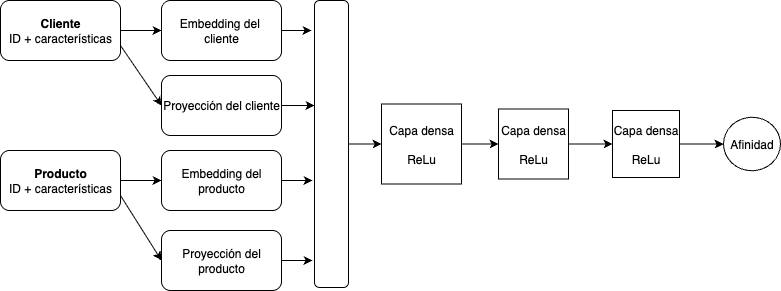
\includegraphics[scale=.5]{./Figures/ncf_hibrido.png}
	\caption{Arquitectura del modelo \textit{Neural Collaborative Filtering} híbrido.}
	\label{fig:ncf_hibrido}
\end{figure}

Durante el entrenamiento, se exploraron diferentes configuraciones de hiperparámetros, incluyendo la dimensión de los embeddings, la cantidad y tamaño de las capas ocultas, la tasa de aprendizaje y la proporción de muestreo negativo. El objetivo fue maximizar el área bajo la curva ROC-AUC sobre un conjunto de validación temporal, buscando un equilibrio entre capacidad predictiva y eficiencia computacional.

El modelo resultante produce un puntaje continuo de afinidad $\hat{y}_{ij}$ para cada combinación cliente–producto. A partir de estos valores se generan listas \textit{Top-$K$} personalizadas, ordenando los productos de mayor a menor probabilidad de interés. Este enfoque híbrido combina la expresividad de las redes neuronales con la capacidad de generalización de los sistemas de recomendación basados en contenido, ofreciendo una mayor flexibilidad para capturar interacciones complejas y atenuar los efectos del arranque en frío.

%----------------------------------------------------------------------------------------

\section{Implementación}

La implementación del sistema de recomendación requirió articular los distintos componentes desarrollados dentro de un flujo de trabajo unificado, reproducible y escalable. Para ello se diseñó un \textit{pipeline} modular que integra los procesos de ingestión, transformación, modelado y evaluación, con soporte para el versionado y monitoreo de artefactos en producción.

\subsection{Diseño del pipeline de procesamiento}

El flujo completo se estructuró en cuatro etapas principales: ingestión, preparación, modelado y predicción.  
En la fase de ingestión se integraron las fuentes de datos transaccionales, digitales y contextuales en un entorno distribuido, garantizando la consistencia de los identificadores y la alineación temporal entre registros. 

Durante la preparación, se aplicaron las transformaciones de limpieza, agregación, codificación y normalización para construir la matriz cliente–producto que sirve de insumo a los modelos.

En la etapa de modelado, se ejecutaron los distintos enfoques desarrollados, almacenando sus métricas, parámetros y versiones.

Finalmente, en la fase de predicción se generaron los puntajes de afinidad y las listas \textit{Top-$K$} para cada cliente, que constituyen la salida principal del sistema.

\subsection{Integración con la infraestructura tecnológica}

La ejecución del pipeline se realizó en la plataforma \texttt{Databricks} \cite{ARTICLE:Databricks}, que permitió procesar grandes volúmenes de datos de forma distribuida utilizando \texttt{PySpark}. Este entorno facilitó la orquestación de tareas, la paralelización de los cálculos y la trazabilidad de los resultados.  

Para la gestión del ciclo de vida de los modelos se empleó \texttt{MLflow} \cite{ARTICLE:MLflow2018}, herramienta que permitió registrar los experimentos, almacenar los parámetros y métricas, y versionar los artefactos generados durante el entrenamiento. Cada ejecución de modelo quedó asociada a un identificador único, lo que posibilita reproducir resultados, comparar configuraciones y recuperar versiones históricas de los modelos entrenados.  

Esta integración entre Databricks y MLflow conformó una infraestructura robusta y escalable, adecuada tanto para la experimentación iterativa como para la implementación de pipelines automatizados.

\subsection{Estrategias de versionado y monitoreo}

Con el fin de garantizar la trazabilidad del sistema, se adoptaron prácticas de control de versiones y monitoreo continuo.  

El código fuente y los scripts asociados al pipeline se gestionaron mediante \texttt{GitHub} \cite{ARTICLE:GitHub}, lo que permitió organizar el desarrollo de manera colaborativa y mantener un historial de cambios documentado.  

Por otro lado, los modelos registrados en \texttt{MLflow} se acompañaron de sus métricas de validación y fecha de generación, posibilitando un seguimiento temporal de su desempeño.  

Además, se establecieron controles de consistencia sobre los datos de entrada y validaciones automáticas del formato de salida, asegurando la estabilidad operativa del sistema en cada ejecución.  

En conjunto, esta arquitectura permitió implementar un flujo de trabajo integrado, auditable y escalable, garantizando la reproducibilidad de los resultados y sentando las bases para la futura incorporación de componentes en producción.


% \definecolor{mygreen}{rgb}{0,0.6,0}
% \definecolor{mygray}{rgb}{0.5,0.5,0.5}
% \definecolor{mymauve}{rgb}{0.58,0,0.82}

% %%%%%%%%%%%%%%%%%%%%%%%%%%%%%%%%%%%%%%%%%%%%%%%%%%%%%%%%%%%%%%%%%%%%%%%%%%%%%
% % parámetros para configurar el formato del código en los entornos lstlisting
% %%%%%%%%%%%%%%%%%%%%%%%%%%%%%%%%%%%%%%%%%%%%%%%%%%%%%%%%%%%%%%%%%%%%%%%%%%%%%
% \lstset{ %
%   backgroundcolor=\color{white},   % choose the background color; you must add \usepackage{color} or \usepackage{xcolor}
%   basicstyle=\footnotesize,        % the size of the fonts that are used for the code
%   breakatwhitespace=false,         % sets if automatic breaks should only happen at whitespace
%   breaklines=true,                 % sets automatic line breaking
%   captionpos=b,                    % sets the caption-position to bottom
%   commentstyle=\color{mygreen},    % comment style
%   deletekeywords={...},            % if you want to delete keywords from the given language
%   %escapeinside={\%*}{*)},          % if you want to add LaTeX within your code
%   %extendedchars=true,              % lets you use non-ASCII characters; for 8-bits encodings only, does not work with UTF-8
%   %frame=single,	                % adds a frame around the code
%   keepspaces=true,                 % keeps spaces in text, useful for keeping indentation of code (possibly needs columns=flexible)
%   keywordstyle=\color{blue},       % keyword style
%   language=[ANSI]C,                % the language of the code
%   %otherkeywords={*,...},           % if you want to add more keywords to the set
%   numbers=left,                    % where to put the line-numbers; possible values are (none, left, right)
%   numbersep=5pt,                   % how far the line-numbers are from the code
%   numberstyle=\tiny\color{mygray}, % the style that is used for the line-numbers
%   rulecolor=\color{black},         % if not set, the frame-color may be changed on line-breaks within not-black text (e.g. comments (green here))
%   showspaces=false,                % show spaces everywhere adding particular underscores; it overrides 'showstringspaces'
%   showstringspaces=false,          % underline spaces within strings only
%   showtabs=false,                  % show tabs within strings adding particular underscores
%   stepnumber=1,                    % the step between two line-numbers. If it's 1, each line will be numbered
%   stringstyle=\color{mymauve},     % string literal style
%   tabsize=2,	                   % sets default tabsize to 2 spaces
%   title=\lstname,                  % show the filename of files included with \lstinputlisting; also try caption instead of title
%   morecomment=[s]{/*}{*/}
% }


%----------------------------------------------------------------------------------------
%	SECTION 1
%----------------------------------------------------------------------------------------
% \section{Análisis del software}
 
% La idea de esta sección es resaltar los problemas encontrados, los criterios utilizados y la justificación de las decisiones que se hayan tomado.

% Se puede agregar código o pseudocódigo dentro de un entorno lstlisting con el siguiente código:

% \begin{verbatim}
% \begin{lstlisting}[caption= "un epígrafe descriptivo"]
% 	las líneas de código irían aquí...
% \end{lstlisting}
% \end{verbatim}

% A modo de ejemplo:

% \begin{lstlisting}[label=cod:vControl,caption=Pseudocódigo del lazo principal de control.]  % Start your code-block

% #define MAX_SENSOR_NUMBER 3
% #define MAX_ALARM_NUMBER  6
% #define MAX_ACTUATOR_NUMBER 6

% uint32_t sensorValue[MAX_SENSOR_NUMBER];		
% FunctionalState alarmControl[MAX_ALARM_NUMBER];	//ENABLE or DISABLE
% state_t alarmState[MAX_ALARM_NUMBER];						//ON or OFF
% state_t actuatorState[MAX_ACTUATOR_NUMBER];			//ON or OFF

% void vControl() {

% 	initGlobalVariables();
	
% 	period = 500 ms;
		
% 	while(1) {

% 		ticks = xTaskGetTickCount();
		
% 		updateSensors();
		
% 		updateAlarms();
		
% 		controlActuators();
		
% 		vTaskDelayUntil(&ticks, period);
% 	}
% }
% \end{lstlisting}



